% !TEX TS-program = lualatex

% required for TexXstudio, an alternative is to change the default bibliography tool 
% in TeXstudio settings (Options > Configure TeXstudio > Build > Default Bibliography Tool)
% !BIB TS-program = biber

% !TeX spellcheck = russian-aot

\documentclass[a4paper,12pt]{article}

% this is required to avoid the conflict on loading xcolor with listing-stata
\PassOptionsToPackage{dvipsnames,svgnames,table}{xcolor}

\usepackage{geometry}
\geometry{left=20.00mm, right=15.00mm, top=20.00mm, bottom=20.00mm}

% to get rid of 'Overfull \hbox...' errors
\usepackage{microtype}

% the support of the large letter in the beginning
%\usepackage{lettrine}

\usepackage{csquotes}

% ------------------------------------------------------------------------------
% Title
% ------------------------------------------------------------------------------

\title{\vspace{-1.5cm}Тестовое задание}
\author{Дмитрий Донецков (ddonetskov@gmail.com)}
\date{\vspace{-5ex}}            % rought equavalent of no date
%\date{\today}

% replacing 'Chapter N' with 'N <Chapter Name>'
%https://tex.stackexchange.com/questions/284893/remove-chapter-from-a-book-text
\usepackage{titlesec}

\titleformat{\chapter}[display]
  {\Huge\bfseries}
  {}
  {0pt}
  {\thechapter.\ }

\titleformat{name=\chapter,numberless}[display]
  {\Huge\bfseries}
  {}
  {0pt}
  {}

% ------------------------------------------------------------------------------
% LUA
% ------------------------------------------------------------------------------

%\usepackage{luacode}

% ------------------------------------------------------------------------------
% TOC
% ------------------------------------------------------------------------------

\usepackage[toc]{multitoc}
\renewcommand*{\multicolumntoc}{2}
\setlength{\columnseprule}{0.5pt}

\usepackage{tocloft}
\renewcommand{\cftsecleader}{\cftdotfill{\cftdotsep}} 
\setlength\cftparskip{-2pt}
\setlength\cftbeforesecskip{1pt}
\setlength\cftaftertoctitleskip{2pt}
\renewcommand{\cftsecfont}{\normalsize}{\sffamily} %\bfseries}

% ------------------------------------------------------------------------------
% Graphics
% ------------------------------------------------------------------------------

\usepackage{graphicx}

% ------------------------------------------------------------------------------
% Figures
% ------------------------------------------------------------------------------

\usepackage{caption}
\usepackage{subcaption}         % subcaptions in figures

% ------------------------------------------------------------------------------
% Lists
% ------------------------------------------------------------------------------

\usepackage{enumitem}           % to regulate space between items

% taken from https://tex.stackexchange.com/questions/300340/topsep-itemsep-partopsep-and-parsep-what-does-each-of-them-mean-and-wha
%\topsep    = vertical space added above and below the list.
%\partopsep = vertical space added above and below the list, but only if the list starts a new paragraph.
%\itemsep   = vertical space added after each item in the list.
%\parsep    = vertical space added after each paragraph in the list.
\setlist[itemize]{topsep=2pt,partopsep=2pt,itemsep=2pt,parsep=2pt}
\setlist[enumerate]{topsep=2pt,partopsep=2pt,itemsep=2pt,parsep=2pt}

% ------------------------------------------------------------------------------
% Tables
% References
% - useful list of various environments: https://tex.stackexchange.com/questions/214840/array-table-tabular-tabularx-longtable-supertabular-longtabu
% 
% ------------------------------------------------------------------------------

\usepackage{array}              % this is to automatically break longer lines of text within cells,
                                % define fixed-width columns
\usepackage{booktabs}           % provides commands to produce heavier lines as table frame
                                % (\toprule, \bottomrule) and lighter lines within a table
                                % (\midrule).
\usepackage{multirow}           % spanning columns across multiple rows
\usepackage{makecell}           % allows different formats inside cells
\usepackage{tabularx}

\renewcommand\arraystretch{1.5} % “stretches” the table vertically, increases space between rows 
% \renewcommand{\tabcolsep}{3pt}  % adjust the space between columns

\renewcommand\theadalign{bc}
\renewcommand\theadfont{\bfseries}
\renewcommand\theadgape{\Gape[4pt]}
\renewcommand\cellgape{\Gape[4pt]}

% ------------------------------------------------------------------------------
% Math (Additional Support)
% ------------------------------------------------------------------------------

\usepackage{amsmath,amsfonts,amssymb,amsthm,mathtools}     % AMS
\usepackage{cancel}             % four different modes of striking through
\usepackage{dsfont}
\usepackage{icomma}             % Smart comma: $0,2$ --- число, $0, 2$ --- перечисление
\usepackage{physics}            % implementation of \abs and \norm
\usepackage{xfrac}              % a better maintained replacement for nicefrac

\DeclareMathOperator*{\D}{\mathbb{D}}   % the dispersion symbol
\DeclareMathOperator*{\E}{\mathbb{E}}   % the expectation symbol

\DeclareMathOperator*{\N}{\mathbb{N}}   % the set of natural numbers
\DeclareMathOperator*{\R}{\mathbb{R}}   % the set of real numbers
\DeclareMathOperator*{\Z}{\mathbb{Z}}   % the set of integers

% e = 2.71...
\newcommand{\e}{\mathrm{e}}

% sign of independence
% \vDash can also be used instead of \models
% \raisebox{}{} is required for vertical alignment
\newcommand{\independent}{\raisebox{0.05em}{\rotatebox[origin=c]{90}{$\models$}}}

% ------------------------------------------------------------------------------
% Russian Language (support thereof)
% ------------------------------------------------------------------------------

%\usepackage[english,russian]{babel}     % multilanguage support
\usepackage{polyglossia}
\setmainlanguage{russian}
\setotherlanguage{english}
\setkeys{russian}{babelshorthands=true}

% ------------------------------------------------------------------------------
% Fonts 
% ------------------------------------------------------------------------------

%\usepackage{fontspec}           % required to load Open Type, True Type fonts

% the next three fonts may be required for the Cyrillic support
%\setmainfont{CMU Serif}
%\setsansfont{CMU Sans Serif}
%\setmonofont{CMU Typewriter Text}

%\setmainfont{Linux Libertine O} % Libertine covers Latin, Hebrew, Greek, and Russian
%\setmonofont{Courier New}

\setmainfont{Times New Roman}
\setromanfont{Times New Roman} 
\setsansfont{Arial} 
\setmonofont[SizeFeatures={Size=11}]{Courier New} 

\newfontfamily{\cyrillicfont}{Times New Roman} 
\newfontfamily{\cyrillicfontrm}{Times New Roman}
\newfontfamily{\cyrillicfonttt}[SizeFeatures={Size=11}]{Courier New}
\newfontfamily{\cyrillicfontsf}{Arial}

\usepackage{euscript}	        % Шрифт Евклид
\usepackage{mathrsfs}         % Красивый матшрифт

\usepackage{fontawesome}

% ------------------------------------------------------------------------------
% Bibliography 
% http://ctan.altspu.ru/macros/latex/exptl/biblatex-contrib/biblatex-gost/doc/biblatex-gost.pdf
% ------------------------------------------------------------------------------

\usepackage[backend=biber,
%style=alphabetic,
%citestyle=authoryear,
citestyle=numeric,
bibstyle=gost-numeric,
sorting=ntvy,
hyperref=true,
dashed=false, 
doi=false, 
eprint=false, 
isbn=false,
url=true,
%backref=true,
maxcitenames=3]{biblatex}

\addbibresource{biblio.bib}

% this is to replace parentheses with square brackets
%\ExecuteBibliographyOptions{parentracker=false}
\makeatletter

\newrobustcmd*{\parentexttrack}[1]{%
  \begingroup
  \blx@blxinit
  \blx@setsfcodes
  \blx@bibopenparen#1\blx@bibcloseparen
  \endgroup}

\AtEveryCite{%
  \let\parentext=\parentexttrack%
  \let\bibopenparen=\bibopenbracket%
  \let\bibcloseparen=\bibclosebracket}

\makeatother

% ------------------------------------------------------------------------------
% Bookmarking, citing, URL's
% ------------------------------------------------------------------------------

\usepackage{bookmark}

% hyperref usually needs to be loaded last
\usepackage{xcolor}
\usepackage{hyperref}
\usepackage{url}

\hypersetup{
    bookmarks=true,
    colorlinks=true,
    linkcolor=blue,
    citecolor=ForestGreen,
    filecolor=red,      
    urlcolor=blue,
    unicode=true
}

\urlstyle{same}

% ------------------------------------------------------------------------------
% Listing
% ------------------------------------------------------------------------------

% downloaded from https://gist.github.com/mcaceresb/b40d6059cf66cc73423f4ddf3f72acda
%\input{listings-stata.tex}

\usepackage{listings}

\lstdefinestyle{python}{
  language          = Python,
  belowcaptionskip  = 1\baselineskip,
  frame             = l,
  xleftmargin       = \parindent,
  basicstyle        = \setmonofont{Consolas}\footnotesize\ttfamily,
  tabsize           = 4,      % Tab size
  showstringspaces  = false,  % Don't underline spaces in strings
  showspaces        = false,  % Don't underline spaces
  breaklines        = true,   % Automatic line breaking
  breakatwhitespace = true,   % Breaks only at white space
  postbreak=\mbox{\textcolor{red}{$\hookrightarrow$}\space},  
  lineskip          = 1.5pt,  % Sparing between lines of code
  % commentstyle      = \color{purple!40!black}\itshape \let\textcolor\textcolordummy
  keywordstyle=\color{blue},
  commentstyle=\color{DarkGreen}\ttfamily,
  % stringstyle=\color{mauve},
  texcl=false
}

\lstdefinestyle{stata}{
%  language          = stata,
  belowcaptionskip  = 1\baselineskip,
  frame             = L,
  xleftmargin       = \parindent,
  basicstyle        = \setmonofont{DejaVu Sans Mono}\footnotesize\ttfamily,
  tabsize           = 4,      % Tab size
  showstringspaces  = false,  % Don't underline spaces in strings
  showspaces        = false,  % Don't underline spaces
  breaklines        = true,   % Automatic line breaking
  breakatwhitespace = true,   % Breaks only at white space.
  lineskip          = 1.5pt,  % Sparing between lines of code
  commentstyle      = \color{black!50}\itshape \let\textcolor\textcolordummy
}

\newcommand{\elochki}[1]{«#1»}
\newcommand{\lapki}[1]{„#1“}

% \lstset{escapechar=@,style=stat_custom}

% ------------------------------------------------------------------------------
% Document
% ------------------------------------------------------------------------------

\begin{document}

\maketitle

\noindent\rule{\textwidth}{2pt}
\tableofcontents
\noindent\rule{\textwidth}{2pt}

\section{Теоретическая задача №1}

Вопрос:

\begin{quote}
Можно ли использовать ковариацию двух признаков для анализа зависимостей между ними?
\end{quote}

Ковариация двух признаков (двух случайных переменных) показывает насколько сильно они меняются \textit{совместно}. Значение ковариации может быть от $-\infty$ до $+\infty$. Если посмотреть на логику формулы (см. ниже) вычисления эмпирического значения ковариации двух случайных переменных $X$ и $Y$, то можно видеть, что это сумма таких произведений, что каждое произведение получает тем большее значение, чем более "синхронно" два признака отклоняются от своих средних значений, а знак ковариации показывает отклоняются ли признаки в одном направлении (положительное значение) или в разных (отрицательное значение):

\begin{align}
\text{Теоретическая ковариация:   } cov(X, Y) &= \E[(X-\E X)(Y-\E Y)] \\
\text{Выборочная ковариация:   } cov(X, Y) &= \frac{1}{n-1} \sum_{i=1}^{n} (x_i - \bar{x})(y_i - \bar{y})
\end{align}

Таким образом, более высокие значения ковариации получаются при более "синхронных" колебаниях переменных, что несёт информацию об их связи, об их зависимости между собой. Но! данную информацию тяжело интерпретировать в силу её ненормализованности (ковариация принимает значения от $-\infty$ до $+\infty$), особенно тяжело её использовать для сравнения силы зависимости между парами разных признаков, например, между двумя парами признаков: рост и вес человека, размер обуви и вес человека. На основе значений ковариаций для этих двух пар невозможно ответить на вопрос, что сильнее связано с весом человека. Данное затруднение исходит из того, что в ковариации содержится размерность исходных признаков, она не свободна от природы измерения самих признаков, которая может быть разной. Поэтому, для \textit{оценки} силы связи между двумя признаками, \textit{сравнения} силы связи между различными парами признаков используют нормализованное значение ковариации - корреляцию, которая уже свободна от размерностей, и принимает своё значение на интервале $[-1; +1]$ вне зависимости от того, множество каких значений могут иметь сами признаки.

\medskip

{\color{red} \faLightbulbO} Что можно добавить в материал: 

\begin{itemize}
\item таблицу сравнения свойств ковариации и корреляции,
% https://keydifferences.com/difference-between-covariance-and-correlation.html
% \item пояснение, что ковариацию теоретически можно использовать для сравнения силы зависимости признаков между собой, если не меняется размерность исследуемых признаков, показать неудобство данного подхода,
\item пояснения, почему ковариация всё равно остаётся очень важным понятием (например, для ковариационных матриц).
% https://stats.stackexchange.com/questions/186276/why-is-covariance-useful
\end{itemize}


\section{Теоретическая задача №2}

Вопрос:

\begin{quote}
Ваш подчинённый обучил модель и получил качество классификации 99\%. Какие бы вопросы про данные и про модель вы бы задали, чтобы убедиться, что модель полезная? Можно считать, что программных багов нет.
\end{quote}

Качество классификации в 99\% выглядит очень хорошим. Естественно, точная интерпретация такой оценки зависит от используемой метрики. Если из контекста задачи неясно какая метрика была использована, то следует задать вопрос об этом вплоть до просьбы показать формулу или фрагмент кода, при помощи которой/которого производилось вычисление метрики. Далее, для ухода от рассмотрения специфики различных метрик (recall, precision, $F_1$, AUC и т.п.), предположим, что речь идёт о доле объектов с верно распознанными классами для них (accuracy).

Итак, качество классификации в 99\% выглядит настолько хорошим, что стоит перепроверить, что полученная модель не является настолько специфичной, что её потом будет нецелесообразно использовать на практике. Другими словами, что нет случая переобучения, смещения оценки, при котором модель будет малоценной для новых объектов. Для такой проверки можно задать следующие вопросы:

\begin{enumerate}
% \item Какой алгоритм классификации был использовал
\item Как распределены объекты по классам? Как удостоверились, что классификатор действительно работает (выдаёт разные значения)? Здесь, необходимо понять, что нет выраженного дисбаланса между классами, когда подавляющее большинство объектов относится к одному классу, а сам классификатор всегда выдаёт значение только одного класса. Другими словами, стоит провести проверку насколько полученная модель лучше dumb-модели. Также, стоит отметить, что в этом случае, несмотря на высокое качество классификации, такое решение "в лоб" может иметь высокую стоимость потерь для оставшегося 1\% случаев, делая модель экономически неэффективной.
\item Каким образом была проведена оценка модели? Здесь, необходимо проверить, что оба множества объектов, используемые для построения модели (тренировки) и её последующей оценки (тестирования), были взяты таким образом, что каждое множество достаточно хорошо представляет собой множество всех возможных объектов (генеральную совокупность). Следует подтолкнуть обучающего к тому, что нужно было использовать техники train/test split, k-fold cross-validation, если они не были использованы.
\end{enumerate}

\medskip

{\color{red} \faLightbulbO} Что можно добавить в материал:
\begin{itemize}
\item пояснения по тому, что метрика accuracy - неполна, есть разные метрики оценки качества классификатора: recall, precision, $F_1$ и т.п.; некоторые из них специфичны, а другие были сконструированы, как интегральные.
\end{itemize}

\section{Практическая задача}

Задание:

\begin{quote}
Напишите функцию one\_hot\_encode(), которая принимает на вход объект pandas.DataFrame и название столбца, и выполняет one-hot-кодирование этого столбца. Гарантируется, что переданный столбец категориальный. Функция должна возвращать новую таблицу (pandas.DataFrame), в которой отсутствует старый столбец, а новые добавлены в конец. Использовать готовые функции для решения этой задачи (например, pandas.get\_dummies()) не разрешается.
\end{quote}

Код функции и её тесты оформлены в виде Jupyter-ноутбука и доступны для просмотра по ссылке \url{https://nbviewer.jupyter.org/github/ddonetskov/misc/blob/master/yp_ds/one_hot_encoding.ipynb#}.

\medskip

{\color{red} \faExclamation} Примечание: реализованная функция не покрывает всех возможных практических случаев, а именно:

\begin{itemize}
\item если есть пропущенные данные в указанном столбце, то функция возвращает исключение \texttt{NotImplementedError}, т.к. логика обработки пропущенных значений может разнится в зависимости от задачи,
\item кодирование выполняется для всех значений в столбце, никакое значение не удаляется, что может порождать проблему с коллинеарностью для соответствующих моделей (например, для линейной регрессии).
\end{itemize}

% https://stats.stackexchange.com/questions/231285/dropping-one-of-the-columns-when-using-one-hot-encoding
% https://datascience.stackexchange.com/questions/27957/why-do-we-need-to-discard-one-dummy-variable/27993#27993

\section{Урок}

Тема урока:

\begin{quote}
Что делает функция pandas.concat()? В каких случаях её используют?
\end{quote}

В библиотеке pandas есть функция \href{https://pandas.pydata.org/pandas-docs/stable/reference/api/pandas.concat.html}{concat}. Её название - это сокращение от английского concatenate, что означает "соединять, сцеплять". Действительно, данная функция используется для соединения двух и более дата фреймов в один. Соединение можно производить как по столбцам и тогда получаемый дата фрейм будет состоять из исходных дата фреймов, \lapki{поставленных} друг на друга (Рис. \ref{fig:concat_vert}), так и по строкам (индексам) и тогда получаемый дата фрейм будет состоять из исходных, \lapki{пристыкованных} боком друг к другу (Рис. \ref{fig:concat_horz}). При этом, в получаемом дата фрейме могут появится совершенно новые элементы, порождённые разницей столбцов или индексов исходных дата фреймов. Данным элементам по умолчанию будет присвоено NaN-значение.

\begin{figure}[h]
  \centering
  \begin{subfigure}[b]{0.45\textwidth}
    \centering
    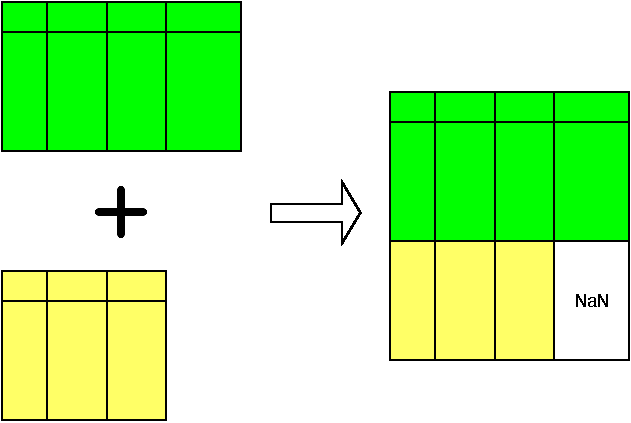
\includegraphics[width=1\linewidth]{image/concat_vert.pdf}
    \caption{соединение по столбцам}
    \label{fig:concat_vert}
  \end{subfigure}
  \hfill
  \begin{subfigure}[b]{0.45\textwidth}
    \centering
    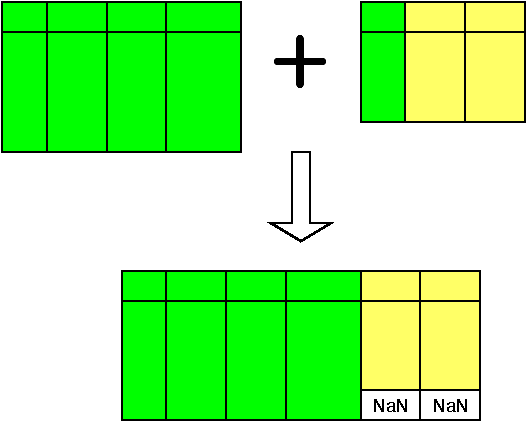
\includegraphics[width=0.85\linewidth]{image/concat_horz.pdf}
    \caption{соединение по индексу}
    \label{fig:concat_horz}
  \end{subfigure}  
  \caption{Соединение двух дата фреймов}
  \label{fig:concat}  
\end{figure}

Рассмотрим на примере оба этих случая. В качестве набора данных будем использовать датасет World Happiness Report для 2015-2017, предоставленный ООН, и который доступен по ссылке \url{https://www.kaggle.com/unsdsn/world-happiness}.

Допустим, вы - исследователь счастья на планете и решили включить в свой анализ и данные из вышеуказанного датасета. Затруднение в том, что на каждый год приходится свой собственный файл, а вам хочется иметь данные в едином дата фрейме. Функция concat поможет здесь. Например, следующим образом можно объединить данные за 2015 и 2016 годы в один итоговый дата фрейм \texttt{whr}:

\begin{lstlisting}[style=python]
whr_2015 = pd.read_csv('data/2015.csv', sep=',')
whr_2016 = pd.read_csv('data/2016.csv', sep=',')

whr_2015['year'] = 2015
whr_2016['year'] = 2016

whr = pd.concat([whr_2015, whr_2016], axis=0, sort=False)
\end{lstlisting}

Полный код с пояснениями размещён по ссылке \url{https://nbviewer.jupyter.org/github/ddonetskov/misc/blob/master/yp_ds/pandas_concat.ipynb}, см. раздел 'Vertical Concatenation'. Обратите внимание!, что те столбцы, которые присутствуют не во всех соединяемых дата фреймах по умолчанию всё равно попадут в итоговый дата фрейм, а элементы, для которых данный столбец ранее не существовал, получат NaN-значения. Таким образом, функция concat придерживается принципа сохранения данных при объединении. {\color{blue} \faCog } Задание: а) найдите такие столбцы для приведённого примера, б) добавьте в пример и файл 2017.csv (сложность объединения его с данными по другим двум годам состоит в том, что для него столбцы при том же смысловом значении получили другие именования, поэтому их предварительно следует переименовать, привести к общему виду).

Приведённый выше пример можно продолжить для случая объединения по индексу. Например, вы решили остановится на анализе данных только 2017 года, но хотели бы дополнить их статистикой по странам. Тогда, можно воспользоваться датасетом по ссылке \url{https://www.kaggle.com/fernandol/countries-of-the-world} и присоединить его данные к данным World Happiness Report для 2017 года. См. полный код в разделе 'Horizontal Concatenation' в том же ноутбуке. {\color{blue} \faCog } Задание: изучите опцию \texttt{ignore\_index} в документации, попробуйте выполнить объединение дата фреймов при \texttt{ignore\_index=True}, и пояснить, почему итоговый результат получится другим?

\begin{lstlisting}[style=python]
whr_2017 = pd.read_csv('data/2017.csv', sep=',')
countries = pd.read_csv('data/countries of the world.csv', sep=',')

# removing spaces around the country names so they would match with whr_2017
countries['Country'] = countries['Country'].str.strip()

# setting the index which will be used to combine two data frame 'horizontally'
whr_2017 = whr_2017.set_index('Country')
countries = countries.set_index('Country')

whr_2017_ext = pd.concat([whr_2017, countries], axis=1, sort=False, ignore_index=False, join='inner')
\end{lstlisting}

{\color{red} \faExclamation} Примечания:

\begin{enumerate}
\item При объединении необходимо отслеживать, что имена общих колонок или значения индекса общих строк - совпадают, иначе полученный результат будет выглядеть, как объединение объектов без общих колонок или значений индекса (данные не объединятся по одним и тем же колонкам или строка).
\item Функция concat также может использоваться и для Series.
\item Функция concat может использоваться для объединения произвольного количества дата фреймов, не только двух, но и трех, четырех и т.д.
\item Для объединения двух датафреймов по индексу можно использовать функции join и merge класса pandas.DataFrame. Они могут быть более удобными в силу своей специализации.
\end{enumerate}

\section{Упражнение (кейс)}

Тема:
\begin{quote}
Классификация для несбалансированных классов. Ошибки первого и второго рода, ROC-кривая, AUC-ROC.
\end{quote}

Разбираемый случай должен быть сконструирован таким образом, чтобы обучающий смог получить понимание, почему а) оценка качества классификатора только по accuracy не является полной, а иногда и проигрышной, б) существуют и другие оценки качества классификатора, включая интегральные. Для этого в качестве бизнес-задачи можно выбрать такую, что для ошибок и первого, и второго рода есть стоимость потерь, а при помощи анализа ROC-кривой следует выбрать наиболее оптимальное, с точки зрения минимизации суммы потерь, значение порога срабатывания классификатора.

Например, можно рассмотреть процесс в поликлинике, когда при помощи бинарного классификатора определяют стоит ли отправить пациента на дальнейшую диагностику, не очень безопасную. При этом стоимость потерь (иски, компенсации и т.п.) при диагностике здорового пациента (по сути, бесполезной диагностики) составляет $C_1$, а стоимость потерь (иски, компенсации и т.п.) при не отправлении больного пациента (по сути, пропущенной диагностики) составляет $C_2$. 

Тогда, датасет может быть сконструирован следующим образом:

\begin{itemize}
\item объект - это пациент с физиологическими и прочими признаками, целевым признаком (не болен/болен),
\item бОльшая часть случаев отмечена, как "не болен", т.к. допустим что заболевание - редкое,
\item граница между больными и небольными пациентами - размытая, в том смысле, что классификатор, насколько он не был бы хорош, всегда будет делать ошибки и первого, и второго рода.
\end{itemize}

Далее, в задании обучающий знакомится с понятиями ошибок, получает представление о том, что accuracy может достигать высоких значений даже при выдачи классификатором всегда "не болен" (dumb или константный классификатор), знакомится с recall/precision/FPR, строит ROC-кривую, вычисляет стоимость потерь в зависимости от выбранного порога срабатывания классификатора. Было бы очень полезно выполнить данное упражнение для разных классификаторов, чтобы сравнить их по метриками качеств, особенно, по ROC-кривой.

{\color{red} \faLightbulbO} Что можно улучшить. Для того, чтобы разбираемый случай (кейс) получился запоминающимся, можно сделать его анекдотичным, указав, что речь идёт о хомячках, которые заболевают тем, что, например, в колесе бегут не вперёд, а назад. Можно взять каких-нибудь литературных персонажей, например, демонов Максвелла из НИИЧАВО, которых нужно заменить классификатором по определению впускать ли посетителя в Институт или нет.

\appendix

\section{Прочее}

\begin{enumerate}
\item Темы и задачи, приведённые выше, могут потребовать бОльшего обсуждения, т.к. они достаточно обширны. В рамках выполнения тестового задания я придерживался принципа минимальной достаточности, но старался показать потенциал развития обучения по той или иной теме.
\item Материал, который предназначен для студентов, лучше оформить не в виде документа подобному текущему, а выложить на сайт, который поддерживает режим совместного редактирования (вики и т.п.). При этом должно выполняться критическое требования - "движок" сайта должен поддерживать оформление математических формул, как это реализовано, например, на Stack Exchange. Но, поскольку у меня нет доступа к платформе, используемой Яндекс.Практикум, то данный материал был пока оформлен в виде текущего PDF-документа (с использованием системы вёрстки \LaTeX).
\end{enumerate}

\end{document}
